\chapter{Community and Topic-level Mediation Results}
\label{sec:appendix-community-mediation}

This appendix provides the full community-level and topic-level mediation results referenced in Sections~\ref{sec:community-mediation-results} and ~\ref{sec:topic-mediation-results}, including pathway selection rationale and complete numerical tables.

\section{Pathway Selection}

The pathways reported here are the treatment-mediator pairs drawn from the three communities $\{0, 1, 2\}$ for which all or nearly all annotation paradigms produced significant ATEs in Section~\ref{sec:community-level-results} (Communities~0, 1, and 2 correspond to White House and Congress, Elections and Campaigns, and Public Health respectively). Of the six ordered pairs among these three communities, four satisfied the minimum presence requirement (at least 50 articles tagged with both the treatment and mediator community) in at least one paradigm and produced non-degenerate mediation decompositions. These are the pathways reported in Table~\ref{tab:mediation_full_communities}: the two configurations with Community~1 as treatment ($1 \to 0$ and $1 \to 2$) and the two contrast configurations with Community~1 as mediator ($0 \to 1$ and $2 \to 1$).

\section{Confounder Reduction Details}

Confounders consist of all community sentiment scores except those of the treatment and mediator communities, reduced in two sequential steps:

\begin{enumerate}
    \item \textbf{Presence filter:} Communities whose sentiment is non-zero in fewer than 50 articles in the treatment subsample are dropped.
    \item \textbf{PCA:} The remaining matrix is reduced via PCA retaining 95\% of variance.
\end{enumerate}

Because this reduction depends only on the treatment subsample, not on ideology labels, it is identical across all annotation paradigms for a given treatment community. The number of retained components therefore varies only by treatment community and not by mediator choice.

\section{Full Community Mediation Results}

Table~\ref{tab:mediation_full_communities} reports Total Effects (TE), Natural Direct Effects (NDE), and Natural Indirect Effects (NIE) under the $Q_{25} \to Q_{75}$ contrast across all five media-split annotation paradigms and all four viable pathways. The $P_{10} \to P_{90}$ contrast yields directionally concordant results.

\begin{table}[h]
\centering
\footnotesize
\begin{tabular}{lcccccc}
\toprule
Annotator & TE & 95\% CI (TE) & NDE & 95\% CI (NDE) & NIE & 95\% CI (NIE) \\
\midrule
\multicolumn{7}{l}{\textit{Community $1 \to 0$ ($N=3{,}628$, sentiment contrast $-0.3$ to $+0.2$)}} \\
\midrule
Human              & $+0.018$ & $[-0.044,\ +0.080]$ & $+0.017$ & $[-0.008,\ +0.043]$ & $+0.001$ & $[-0.005,\ +0.010]$ \\
Fine-tuned RoBERTa & $+0.013$ & $[-0.051,\ +0.077]$ & $+0.009$ & $[-0.017,\ +0.034]$ & $+0.004$ & $[-0.004,\ +0.010]$ \\
GPT (baseline)     & $+0.039$ & $[-0.013,\ +0.091]$ & $\mathbf{+0.039^*}$ & $\mathbf{[+0.018,\ +0.060]}$ & $-0.000$ & $[-0.003,\ +0.009]$ \\
Fine-tuned GPT     & $+0.010$ & $[-0.053,\ +0.073]$ & $+0.003$ & $[-0.022,\ +0.028]$ & $+0.007$ & $[-0.000,\ +0.014]$ \\
Llama-3.3-70B      & $\mathbf{+0.065^*}$ & $\mathbf{[+0.001,\ +0.129]}$ & $\mathbf{+0.069^*}$ & $\mathbf{[+0.041,\ +0.093]}$ & $-0.003$ & $[-0.006,\ +0.009]$ \\
\midrule
\multicolumn{7}{l}{\textit{Community $1 \to 2$ ($N=3{,}628$, sentiment contrast $-0.3$ to $+0.2$)}} \\
\midrule
Human              & $+0.018$ & $[-0.042,\ +0.078]$ & $+0.014$ & $[-0.010,\ +0.042]$ & $+0.005$ & $[-0.001,\ +0.009]$ \\
Fine-tuned RoBERTa & $+0.014$ & $[-0.046,\ +0.074]$ & $+0.007$ & $[-0.016,\ +0.033]$ & $+0.007$ & $[-0.001,\ +0.009]$ \\
GPT (baseline)     & $+0.039$ & $[-0.011,\ +0.089]$ & $\mathbf{+0.037^*}$ & $\mathbf{[+0.018,\ +0.060]}$ & $+0.002$ & $[-0.001,\ +0.007]$ \\
Fine-tuned GPT     & $+0.005$ & $[-0.056,\ +0.065]$ & $-0.000$ & $[-0.022,\ +0.027]$ & $+0.005$ & $[-0.002,\ +0.007]$ \\
Llama-3.3-70B      & $\mathbf{+0.067^*}$ & $\mathbf{[+0.005,\ +0.129]}$ & $\mathbf{+0.067^*}$ & $\mathbf{[+0.041,\ +0.092]}$ & $-0.000$ & $[-0.001,\ +0.009]$ \\
\midrule
\multicolumn{7}{l}{\textit{Community $0 \to 1$ ($N=2{,}743$, sentiment contrast $-0.2$ to $+0.1$)}} \\
\midrule
Human              & $-0.021$ & $[-0.083,\ +0.041]$ & $\mathbf{-0.030^*}$ & $\mathbf{[-0.046,\ -0.002]}$ & $+0.009$ & $[-0.012,\ +0.010]$ \\
Fine-tuned RoBERTa & $-0.029$ & $[-0.091,\ +0.034]$ & $\mathbf{-0.030^*}$ & $\mathbf{[-0.047,\ -0.004]}$ & $+0.001$ & $[-0.012,\ +0.008]$ \\
GPT (baseline)     & $-0.013$ & $[-0.066,\ +0.041]$ & $-0.012$ & $[-0.028,\ +0.009]$ & $\mathbf{-0.001^*}$ & $\mathbf{[-0.021,\ -0.003]}$ \\
Fine-tuned GPT     & $-0.026$ & $[-0.089,\ +0.036]$ & $\mathbf{-0.034^*}$ & $\mathbf{[-0.052,\ -0.006]}$ & $+0.008$ & $[-0.012,\ +0.010]$ \\
Llama-3.3-70B      & $-0.014$ & $[-0.077,\ +0.050]$ & $-0.003$ & $[-0.022,\ +0.024]$ & $\mathbf{-0.011^*}$ & $\mathbf{[-0.031,\ -0.008]}$ \\
\midrule
\multicolumn{7}{l}{\textit{Community $2 \to 1$ ($N=1{,}116$, sentiment contrast $-0.3$ to $+0.1$)}} \\
\midrule
Human              & $-0.081$ & $[-0.182,\ +0.020]$ & $\mathbf{-0.081^*}$ & $\mathbf{[-0.122,\ -0.039]}$ & $+0.000$ & $[-0.011,\ +0.011]$ \\
Fine-tuned RoBERTa & $-0.052$ & $[-0.163,\ +0.059]$ & $\mathbf{-0.055^*}$ & $\mathbf{[-0.109,\ -0.017]}$ & $+0.003$ & $[-0.006,\ +0.019]$ \\
GPT (baseline)     & $-0.074$ & $[-0.160,\ +0.012]$ & $\mathbf{-0.085^*}$ & $\mathbf{[-0.120,\ -0.055]}$ & $+0.011$ & $[-0.009,\ +0.015]$ \\
Fine-tuned GPT     & $-0.071$ & $[-0.179,\ +0.037]$ & $\mathbf{-0.059^*}$ & $\mathbf{[-0.114,\ -0.026]}$ & $-0.012$ & $[-0.011,\ +0.011]$ \\
Llama-3.3-70B      & $-0.087$ & $[-0.182,\ +0.008]$ & $\mathbf{-0.104^*}$ & $\mathbf{[-0.141,\ -0.065]}$ & $+0.017$ & $[-0.014,\ +0.013]$ \\
\bottomrule
\end{tabular}
\caption{Community-level mediation results ($Q_{25} \to Q_{75}$ contrast) across media-split annotation paradigms. $^*$Significant at 95\% (CI excludes zero).}
\label{tab:mediation_full_communities}
\end{table}

\section{Topic Mediation Results For Treatment Donald Trump}

\begin{table}[ht]
  \centering
  \sisetup{table-format=+1.3}
  \begin{tabular}{llS[table-format=+1.3]S[table-format=+1.3]S[table-format=+1.3]S[table-format=+1.3]S[table-format=+1.3]}
    \toprule
    \textbf{Paradigm} & \textbf{Contrast} &
      {\textbf{TE}} &
      {\textbf{CI lower}} & {\textbf{CI upper}} &
      {\textbf{NDE}} & {\textbf{NIE}} \\
    \midrule
    Human
      & $Q25 \to Q75$  & +0.135 & -0.001 & +0.270 & +0.124 & +0.010 \\
    Human
      & $P10 \to P90$  & +0.314 & -0.002 & +0.630 & +0.300 & +0.014 \\
    \addlinespace
    Fine-tuned RoBERTa
      & $Q25 \to Q75$  & {$\mathbf{+0.154^{*}}$} & {$\mathbf{+0.016}$} & {$\mathbf{+0.292}$} & +0.135 & +0.019 \\
    Fine-tuned RoBERTa
      & $P10 \to P90$  & {$\mathbf{+0.359^{*}}$} & {$\mathbf{+0.038}$} & {$\mathbf{+0.681}$} & +0.320 & +0.040 \\
    \addlinespace
    GPT-4o-mini (baseline)
      & $Q25 \to Q75$  & {$\mathbf{+0.255^{*}}$} & {$\mathbf{+0.155}$} & {$\mathbf{+0.355}$} & +0.249 & +0.006 \\
    GPT-4o-mini (baseline)
      & $P10 \to P90$  & {$\mathbf{+0.595^{*}}$} & {$\mathbf{+0.362}$} & {$\mathbf{+0.828}$} & +0.585 & +0.010 \\
    \addlinespace
    Fine-tuned GPT-4o-mini
      & $Q25 \to Q75$  & {$\mathbf{+0.158^{*}}$} & {$\mathbf{+0.022}$} & {$\mathbf{+0.293}$} & +0.141 & +0.017 \\
    Fine-tuned GPT-4o-mini
      & $P10 \to P90$  & {$\mathbf{+0.368^{*}}$} & {$\mathbf{+0.052}$} & {$\mathbf{+0.684}$} & +0.335 & +0.032 \\
    \addlinespace
    Llama-3.3-70B
      & $Q25 \to Q75$  & {$\mathbf{+0.316^{*}}$} & {$\mathbf{+0.187}$} & {$\mathbf{+0.445}$} & +0.316 & -0.000 \\
    Llama-3.3-70B
      & $P10 \to P90$  & {$\mathbf{+0.737^{*}}$} & {$\mathbf{+0.437}$} & {$\mathbf{+1.037}$} & +0.741 & -0.004 \\
    \bottomrule
  \end{tabular}
  \caption{Total Effect (TE) of Donald Trump sentiment on ideology label for
    two percentile contrasts. $N = \num{1424}$ articles. All five paradigms agree on a
    positive direction; four of five reach 95\%
    significance under both contrasts (marked $^*$), with Human narrowly missing. The direct channel (NDE) dominates the indirect channel (NIE) in all paradigms.}
  \label{tab:te-trump}
\end{table}

\section{Random-Split Community Mediation Decompositions}

This section collects the mediation decomposition figures for the three pathways not embedded in Section~\ref{sec:random-community-mediation-results}. The corresponding numerical values are reported in Table~\ref{tab:random-community-mediation}.

\begin{figure}[h!]
    \centering
    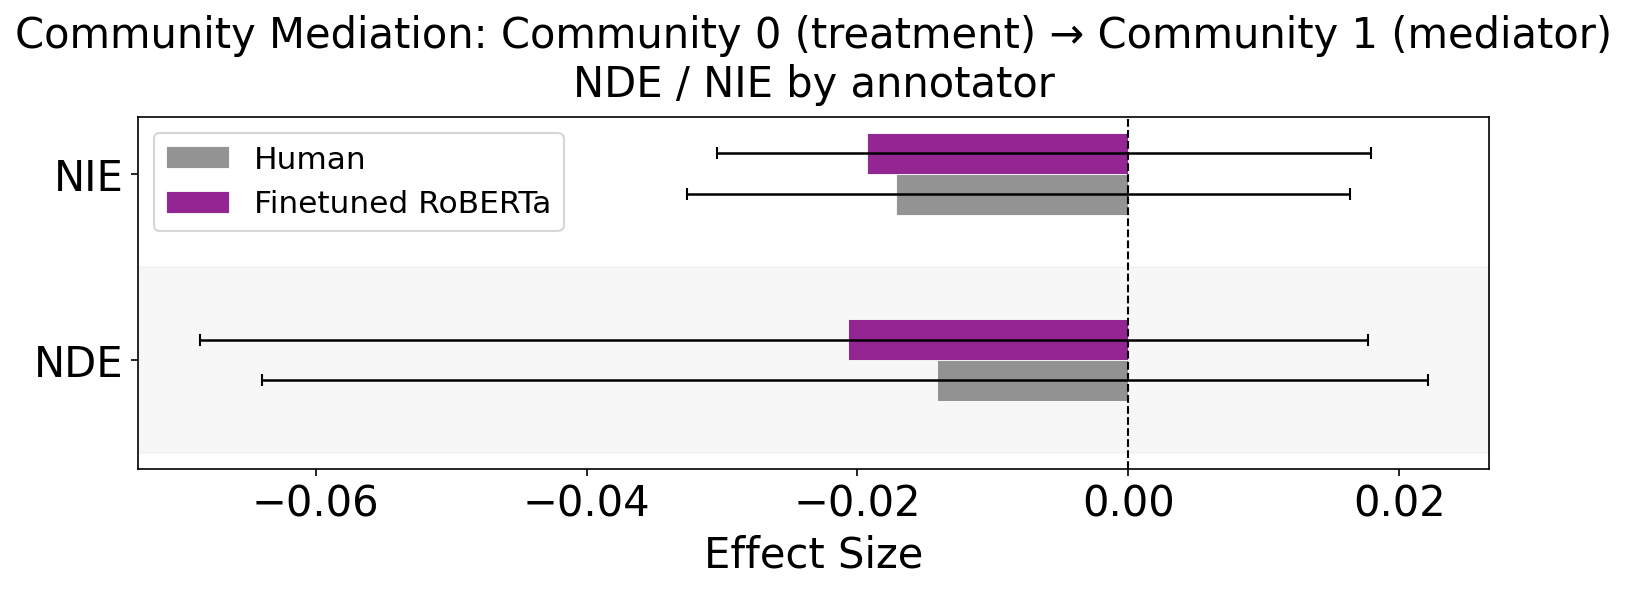
\includegraphics[width=0.7\textwidth]{sections/images/causal_analysis/random_split/mediation_community_0_1.png}
    \caption{Mediation decomposition for the Community $0 \to 1$ pathway under the AllSidesV2 random split ($N = \num{1022}$), $Q_{25} \to Q_{75}$ contrast, Human and Fine-tuned RoBERTa paradigms.}
    \label{fig:random-mediation-0-1}
\end{figure}

\begin{figure}[h!]
    \centering
    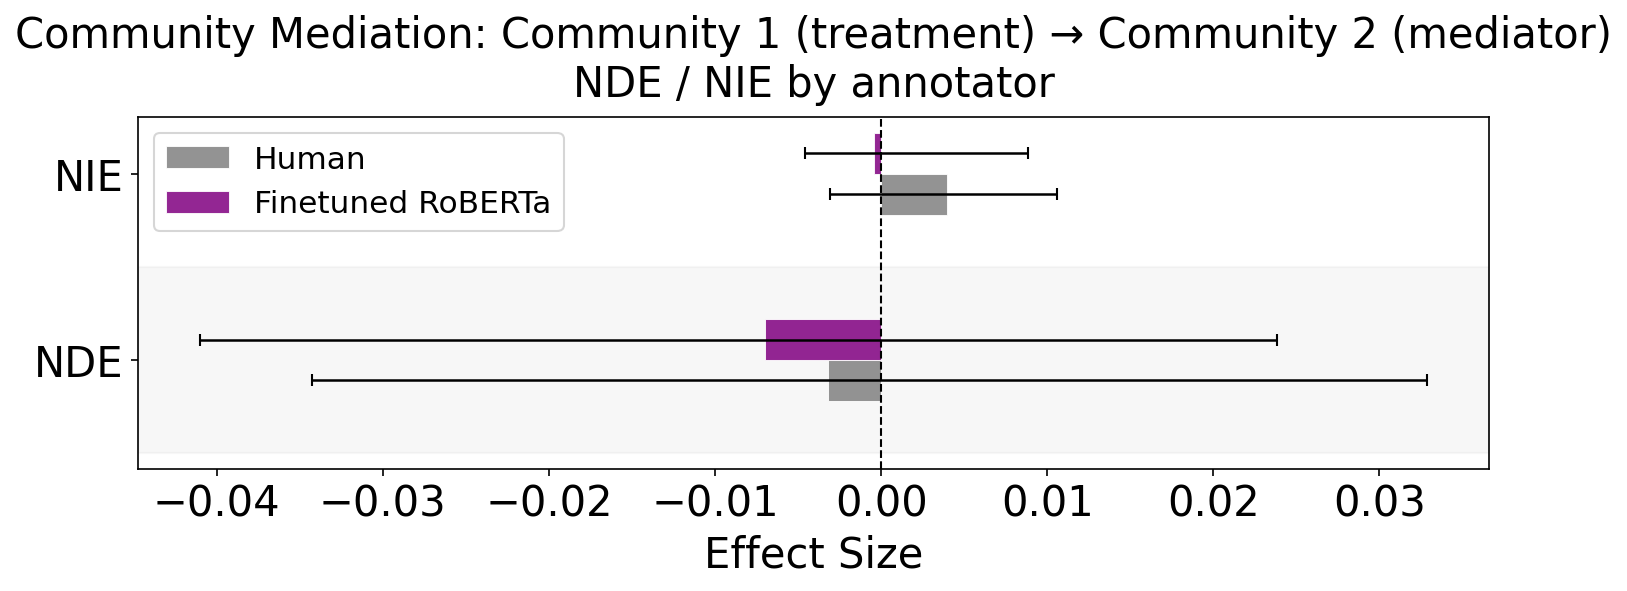
\includegraphics[width=0.7\textwidth]{sections/images/causal_analysis/random_split/mediation_community_1_2.png}
    \caption{Mediation decomposition for the Community $1 \to 2$ pathway under the AllSidesV2 random split ($N = \num{1551}$), $Q_{25} \to Q_{75}$ contrast, Human and Fine-tuned RoBERTa paradigms.}
    \label{fig:random-mediation-1-2}
\end{figure}

\begin{figure}[h!]
    \centering
    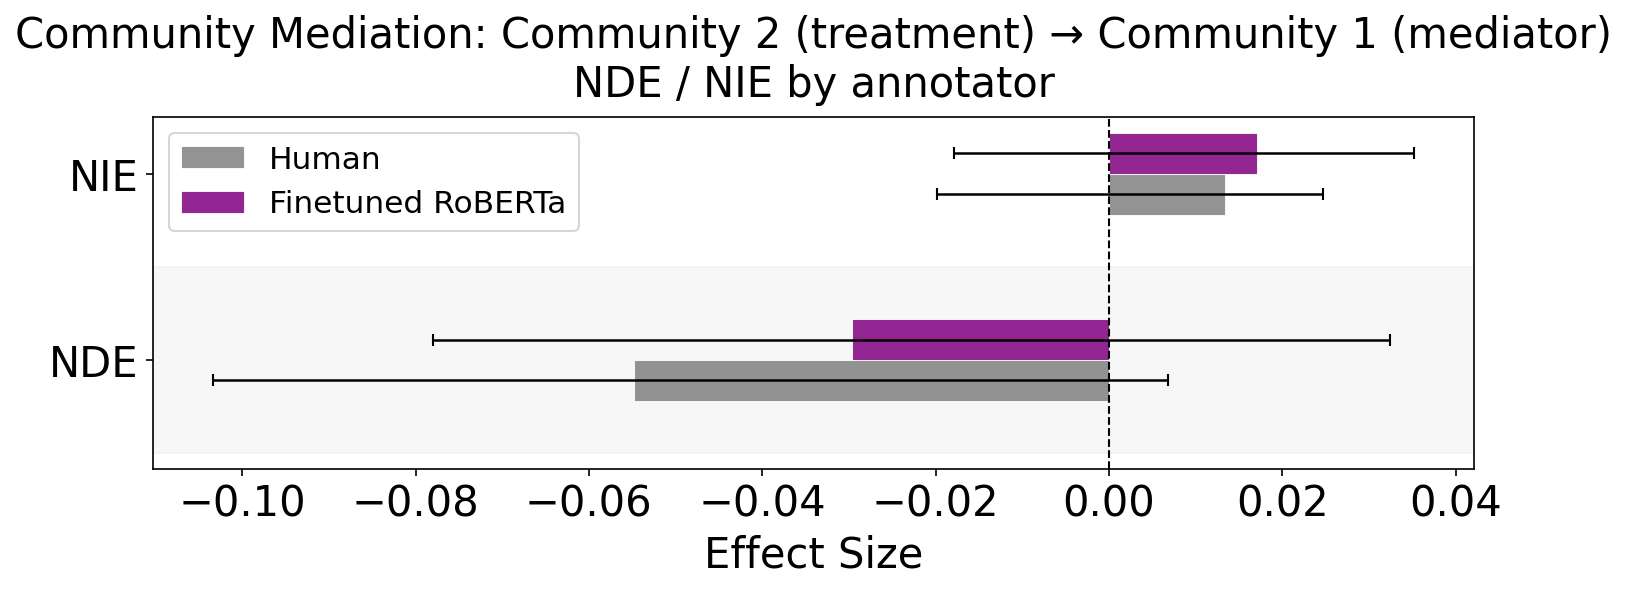
\includegraphics[width=0.7\textwidth]{sections/images/causal_analysis/random_split/mediation_community_2_1.png}
    \caption{Mediation decomposition for the Community $2 \to 1$ pathway under the AllSidesV2 random split ($N = 536$), $Q_{25} \to Q_{75}$ contrast, Human and Fine-tuned RoBERTa paradigms.}
    \label{fig:random-mediation-2-1}
\end{figure}
